\documentclass[oneside,a4paper,14pt]{extarticle}
\usepackage[a4paper,letterpaper,top=20mm,bottom=20mm,left=20mm,right=10mm]{geometry}
\usepackage[russian]{babel}
\usepackage{indentfirst}
\usepackage{amsmath}
\usepackage{amsfonts}
\usepackage{amsthm}
\usepackage{graphicx}
\usepackage{caption}
\usepackage{titlesec}
\usepackage{minted, fancyvrb}

\titleformat{\section} {\normalsize\bfseries} {\thesection} {1em} {}
\titleformat{\subsection} {\normalsize\bfseries} {\thesubsection} {1em} {}
\titleformat{\subsubsection} {\normalsize\bfseries} {\thesubsection} {1em} {}
\renewcommand\baselinestretch{1.45}\normalsize
\setlength{\parindent}{1.25cm}

\begin{document}

\newpage
\thispagestyle{empty}
\begin{center}
	МИНИСТЕРСТВО НАУКИ И ВЫСШЕГО ОБРАЗОВАНИЯ РОССИЙСКОЙ ФЕДЕРАЦИИ ФЕДЕРАЛЬНОЕ ГОСУДАРСТВЕННОЕ БЮДЖЕТНОЕ ОБРАЗОВАТЕЛЬНОЕ УЧРЕЖДЕНИЕ ВЫСШЕГО ОБРАЗОВАНИЯ\\
	«ВЯТСКИЙ ГОСУДАРСТВЕННЫЙ УНИВЕРСИТЕТ»\\
	Институт математики и информационных систем\\
	Факультет автоматики и вычислительной техники\\
	Кафедра электронных вычислительных машин
\end{center}
\vspace{10mm}

\hfill
\begin{tabular}{l}
  \footnotesize Дата сдачи на проверку: \\
  \footnotesize <<\rule[-1mm]{5mm}{0.10mm}\/>>\rule[-1mm]{20mm}{0.10mm}\ 2025 г.\\
  \footnotesize Проверено: \\
  \footnotesize <<\rule[-1mm]{5mm}{0.10mm}\/>>\rule[-1mm]{20mm}{0.10mm}\ 2025 г. \\
\end{tabular}
\vfill

\begin{center}
  ГРАФЫ. СВЯЗНОСТЬ ГРАФОВ.\\
	Отчёт по лабораторной работе №5\\
	по дисциплине\\
	<<Дискретная математика>>\\
\end{center}
\vspace{25mm}
\noindent
\begin{tabular}{ll}
	Разработал студент гр. ИВТб-1301-05-00 & \rule[-1mm]{30mm}{0.10mm}\,/Черкасов А. А./   \\
	                                       & \hspace{8mm}\footnotesize(подпись)            \\
	Проверила преподаватель                & \rule[-1mm]{30mm}{0.10mm}\,/Пахарева И. В./ \\
	                                       & \hspace{8mm}\footnotesize(подпись)            \\
\end{tabular}

\noindent
  \begin{tabular}{lp{58mm}r}
    Работа защищена &  & <<\rule[-1mm]{5mm}{0.10mm}\/>>\rule[-1mm]{30mm}{0.10mm}\ 2025 г.
  \end{tabular}
  \vfill

\begin{center}
	Киров\\
	2025
\end{center}

\newpage\thispagestyle{plain}

\section*{Цель}

Цель работы: изучить представление ориентированного графа с помощью матрицы инцидентности, освоить преобразование этой матрицы в матрицу смежности, сформировать матрицу достижимости (матрицу связности) и проверить условие односторонней связности заданного графа.

\section*{Задание}
\begin{itemize}
	\item[$-$] Ориентированный граф \(G\) задаётся матрицей инцидентности, записанной в файле \texttt{input.txt}. Ограничить размерность: число вершин и число дуг (ребер) \(\ge 4\).
	\item[$-$] Сформировать из матрицы инцидентности матрицу смежности \(A\).
	\item[$-$] По матрице смежности \(A\) построить матрицу достижимости \(R\) (матрицу связности) методом последовательного умножения или алгоритмом Вархалла–Флойда.
	\item[$-$] На основании матрицы достижимости определить, является ли граф односторонне связным: для любой пары вершин \(u,v\) должно выполняться \(\bigl(R_{uv}=1\bigr)\) или \(\bigl(R_{vu}=1\bigr)\).
\end{itemize}

\section*{Решение}

Схема алгоритма решения представлена на рисунках 1.1, 1.2 и 1.3. Примеры работы программы представлены на рисунках 2.1 и 2.2. Исходный код представлен в приложении A1.

\clearpage
\begin{figure}[H]
	\centering
	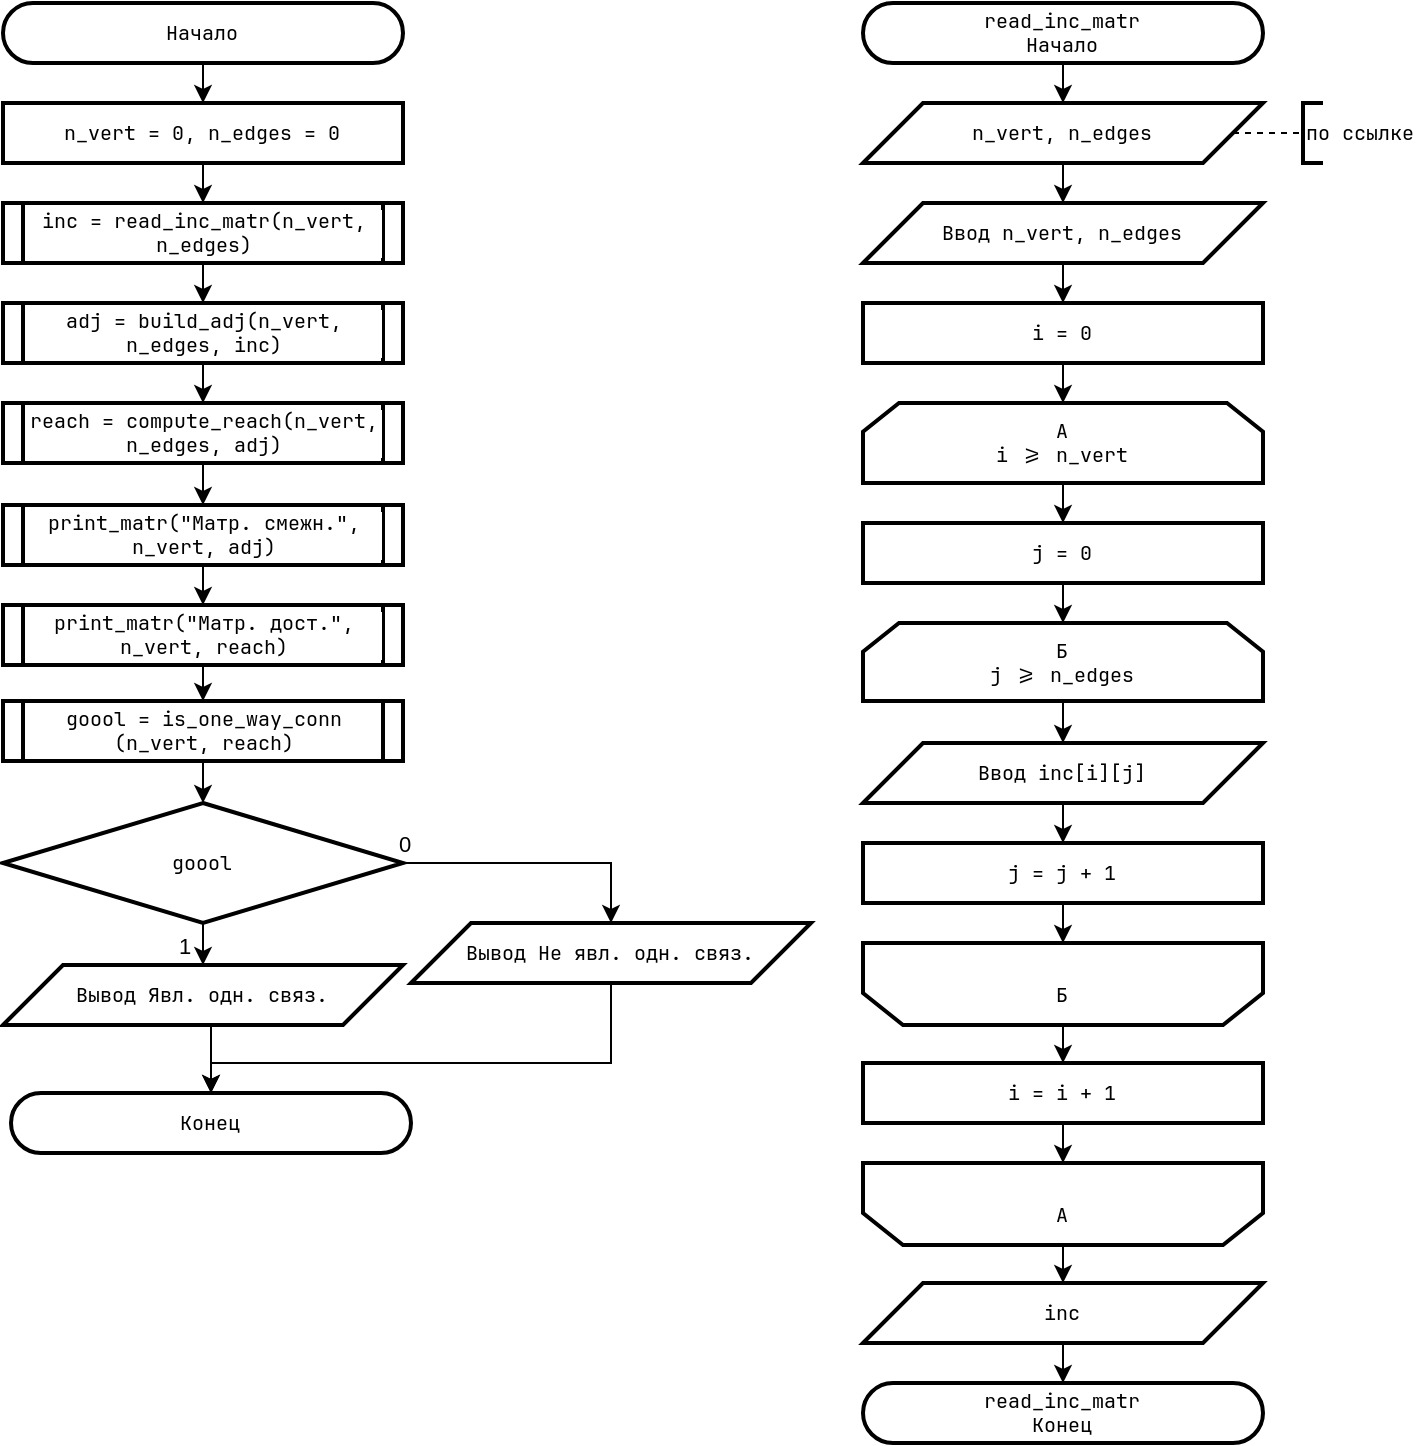
\includegraphics[width=0.9\textwidth]{pics/flowchart1.png}
	\caption*{Рисунок 1.1 - Схема алгоритма основной программы и подпрограммы чтения матрицы инцидентности.}
\end{figure}

\clearpage
\begin{figure}[H]
	\centering
	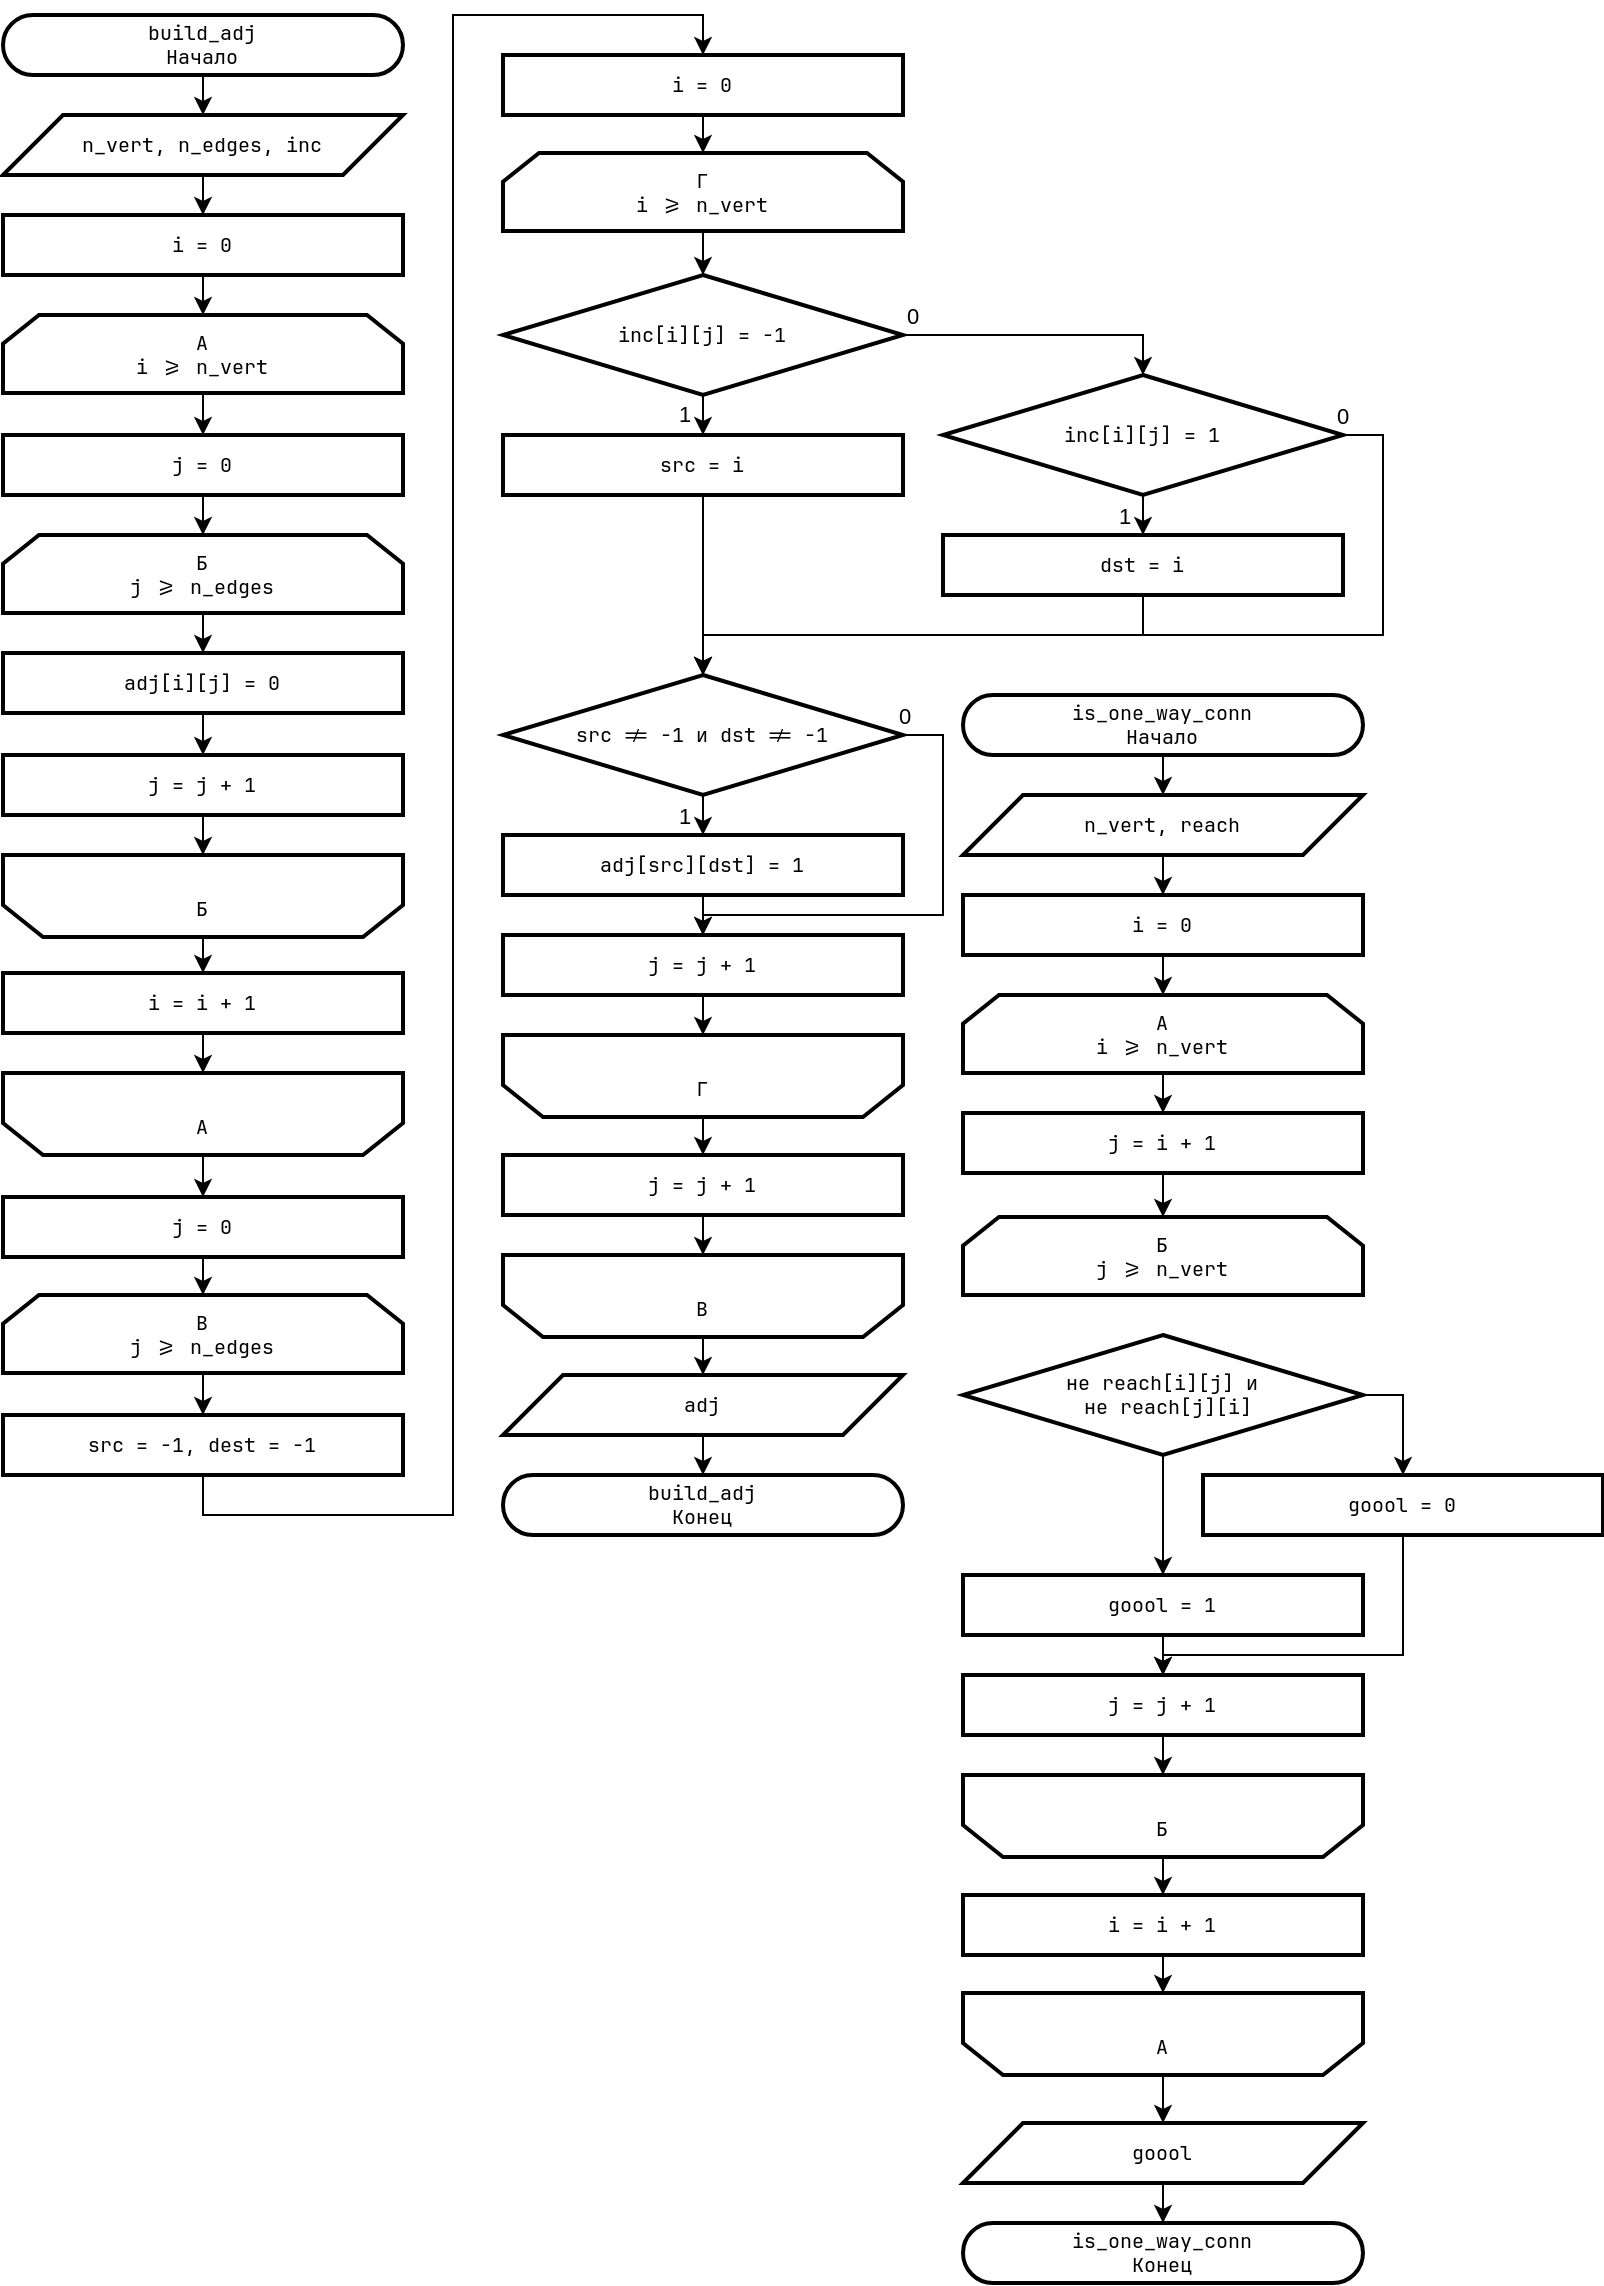
\includegraphics[height=0.9\textheight]{pics/flowchart2.png}
	\caption*{Рисунок 1.2 - Схема алгоритма основной программы и подпрограммы чтения матрицы инцидентности.}
\end{figure}

\clearpage
\begin{figure}[H]
	\centering
	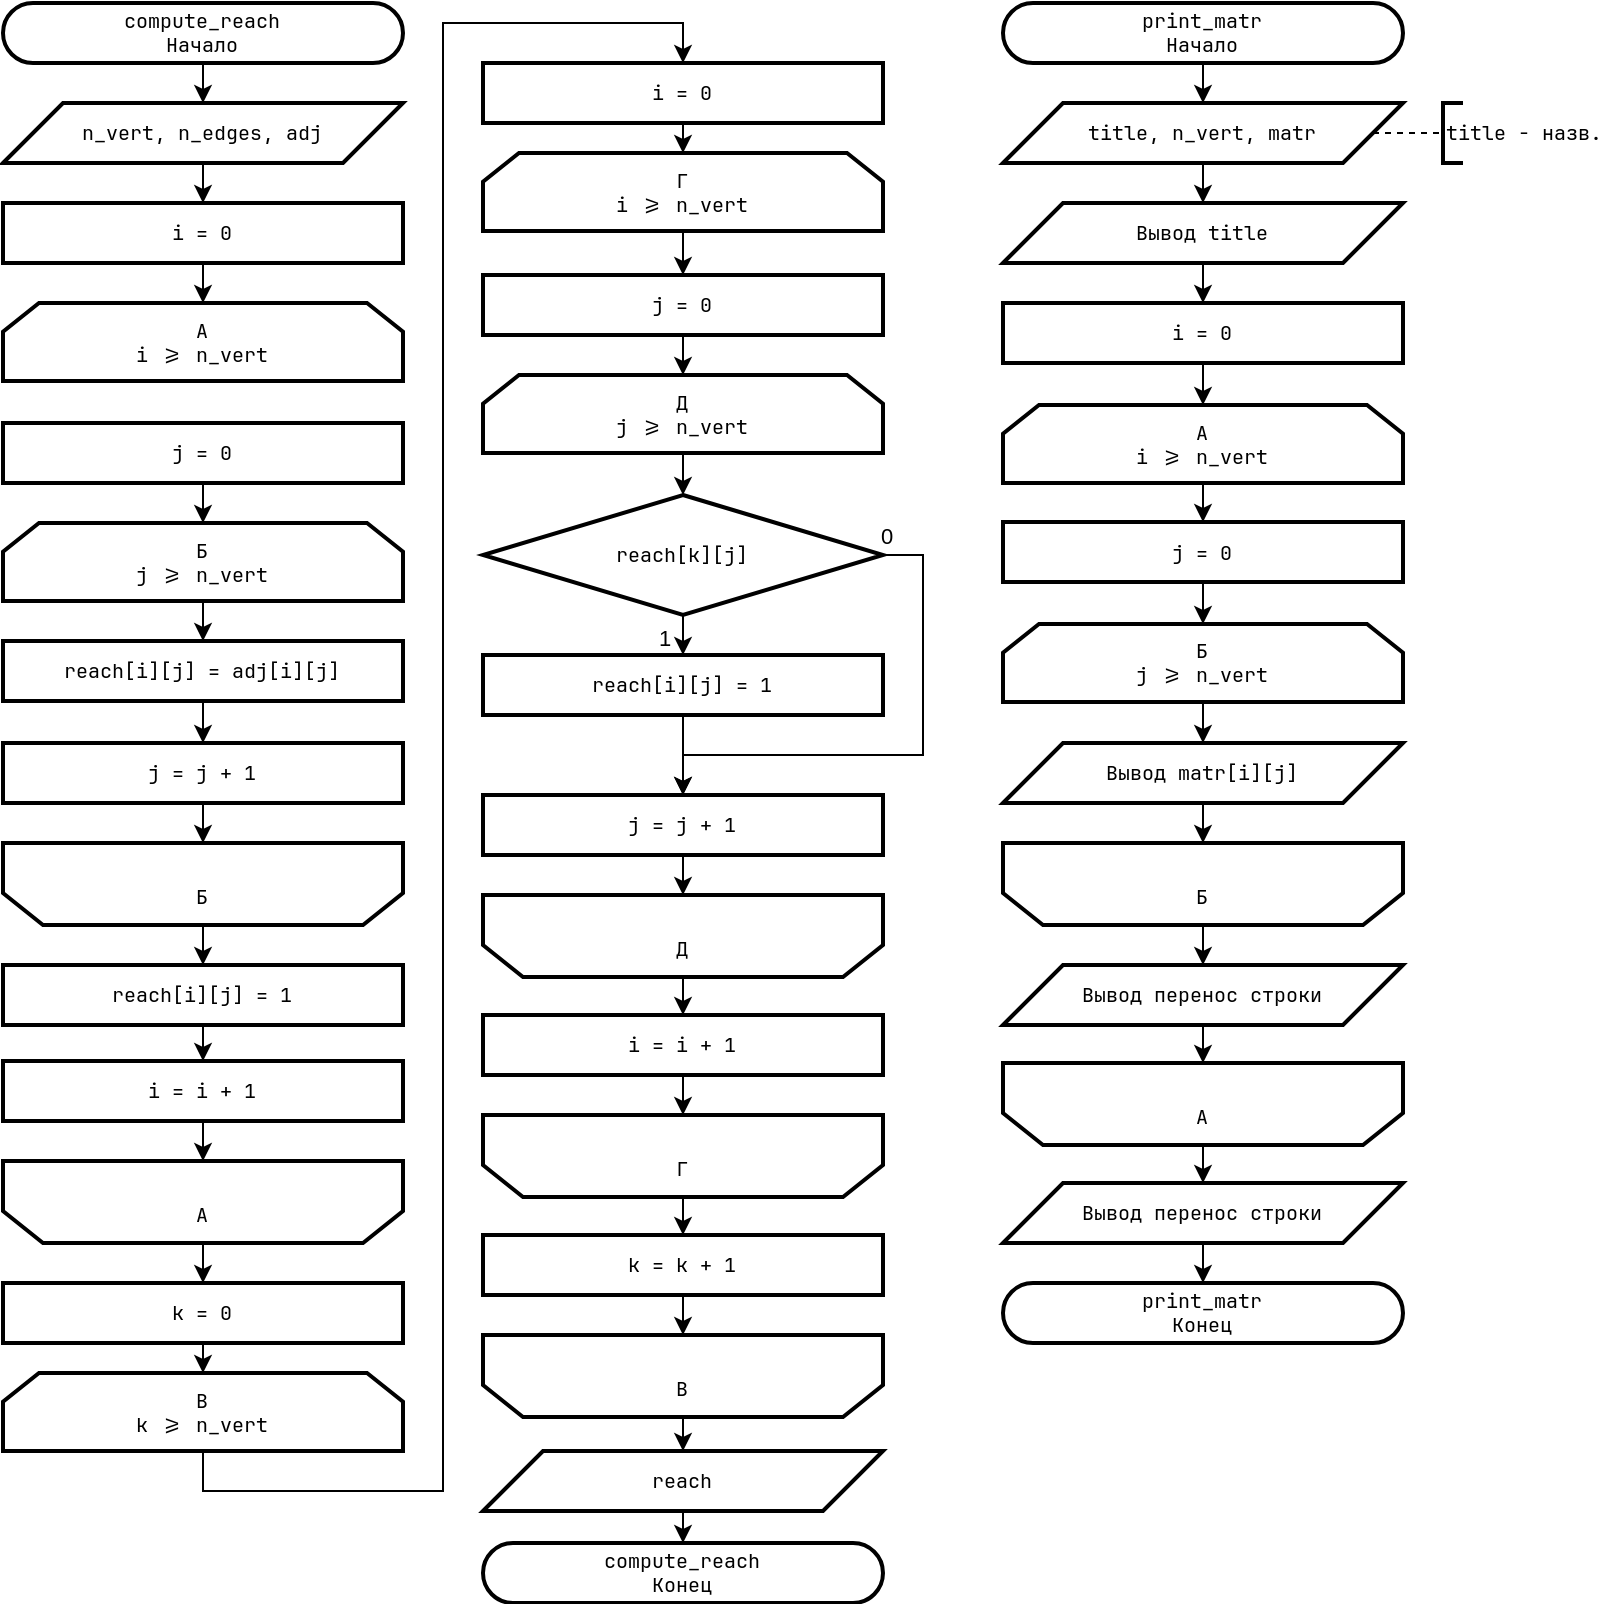
\includegraphics[width=0.9\textwidth]{pics/flowchart3.png}
	\caption*{Рисунок 1.3 - Схема алгоритма основной программы и подпрограммы чтения матрицы инцидентности.}
\end{figure}

\clearpage
\begin{figure}[H]
	\centering
	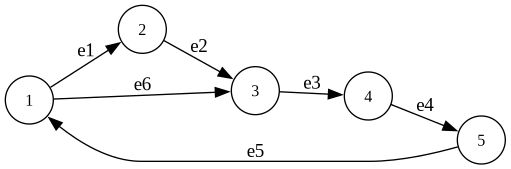
\includegraphics[width=0.75\textwidth]{pics/graph.png}
	\caption*{Рисунок 2.1 - Граф.}
\end{figure}

\begin{figure}[H]
	\centering
	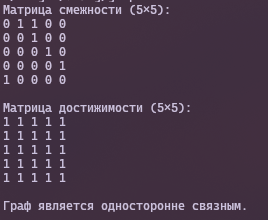
\includegraphics[width=0.6\textwidth]{pics/screen.png}
	\caption*{Рисунок 2.2 - Пример работы программы.}
\end{figure}

\clearpage
\section*{Вывод}

В ходе выполнения лабораторной работы были отработаны навыки работы с матрицей инцидентности для представления ориентированного графа и преобразования её в матрицу смежности. Далее с помощью алгоритма построения матрицы достижимости (матрицы связности) удалось проверить, является ли заданный граф односторонне связным. Реализованная программа корректно читает матрицу инцидентности из файла \texttt{input.txt}, формирует матрицу смежности, вычисляет матрицу достижимости и делает заключение о наличии односторонней связности. Работа способствовала пониманию фундаментальных операций над графами и закреплению алгоритмов поиска путей в ориентированных графах.

\setminted{style = rainbow_dash, fontsize = \small} % https://pygments.org/styles/

\clearpage
\section*{Приложение А1. Исходный код}
\inputminted{cpp}{code/src/main.cpp}

\clearpage
\inputminted{cpp}{code/src/graphviz.hpp}

\inputminted{cpp}{code/src/graphviz.cpp}

\end{document}
